\documentclass{article}
\usepackage[a4paper, left=2cm, right=2cm, top=2.5cm, bottom=2.5cm]{geometry}
\usepackage{graphicx} % Required for inserting images
\usepackage{xcolor} % Required for color commands

\title{PPO}
\author{Jan Janoušek}
\date{June 2025}

\newcommand{\todo}[1]{}
\renewcommand{\todo}[1]{{\color{red} TO DO: {#1}}}

\begin{document}

\maketitle

\section{Introduction}
\subsection{Task definition}
Our goal in this project is to compare several sampling methods (two-stage cluster random sampling) and their sample means and variances of the mean estimators. We are working with \texttt{soildata} dataset consisting of information about minerals in the soil in the natural reservation Barro Colorado Island in Panama in an observational window of $1000m \times 500 m$. We also have data about squares (pixels) with a side length of $ 20 m$; thus, we have $1,250$ pixels in our dataset.


The dataset consists of geographical location ($x$ and $y$ axes) and concentration of several minerals, including Aluminium, Calcium, Iron, Copper, etc. Our goal is to work with the content of \texttt{Cu}, i.e., Copper.

In addition, there will be some places with missing data (so-called white pixels), we can choose these points ourselves. We will choose these points randomly and only set the percentage of white pixels.

Our goal is to compare these sampling methods:
\begin{enumerate}
    \item Two-stage cluster random sampling with primary units being selected with probability proportional to size, with replacement. Secondary units selected by simple random sampling.
    \item Two-stage cluster random sampling with both primary and secondary units being selected by simple random sampling.
    \item Stratified two-stage cluster random sampling, where the clusters within a stratum are selected by simple random sampling as well as secondary units within the clusters.
    \item Simple random sampling of the population units.
\end{enumerate}
with various sample sizes and various fractions of white pixels.

In the first part, we will provide formulae and illustration plots for a specific sample size and fraction of white pixels. In the second part, we will provide numerical data about differences in means and variances of mean estimators for different sample sizes and different fractions of white pixels.


\subsection{Data exploration}
We have a dataset with $1250$ observations. The mean is $7072.98$ with minimum of $1252$, $25\%$--quantile $5807.5$, median of $6901$, $75\%$-quantile of $8131.75$ and maximum of $15119.$ Our goal is to estimate the mean and also the variance of the estimator.

The heatmap of the concentration can be seen in Figure~\ref{fig:cu_heatmap}. We can see stripes of high concentration towards the east of the observation window, going all the way from the south end to the north end of the window, and stripes of low concentration in the middle of the window, again going all the way from south to north.

\begin{figure}
    \centering
    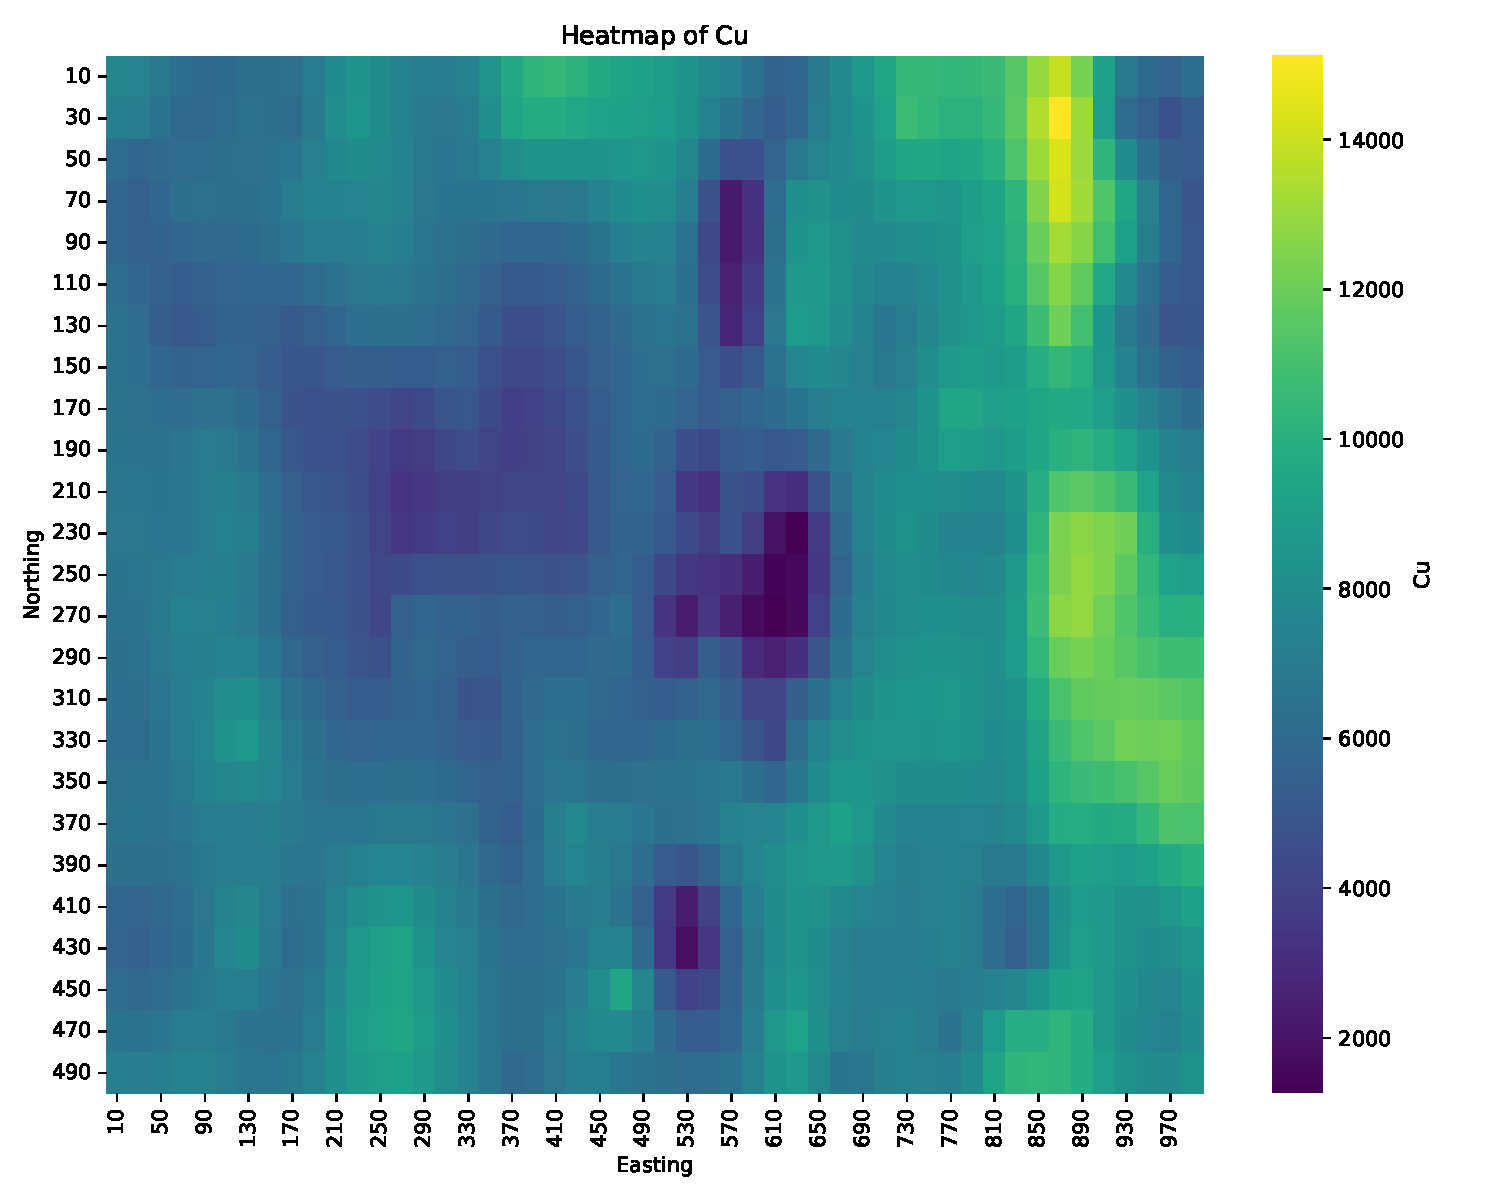
\includegraphics[width=\linewidth]{img/cu_heatmap.pdf}
    \caption{Heatmap of the content of copper}
    \label{fig:cu_heatmap}
\end{figure}
\section{Methodologic part}
For illustration purposes, let us use the following constants:
\begin{itemize}
    \item Percentage of white pixels $0$ (for illustration purposes, we will include this later)
    \item Total number of clusters $N=20$
    \item Number of strata $N_{strata}=5$
    \item Number of selected clusters $n_{psu}=6$
    \item Number of selected secondary units $n_{ssu} = 5$
    \item Number of clusters per stratum $N_{CinS} = 2$
    \item Number of selected population units in assignment $D$: $n_D=30$ (we will always use $n_D = n_{psu} n_{ssu}$)
    \item Number of total secondary units in cluster $i$: $M_i$
    \item Number of selected secondary units in cluster $i$: $m_i$ ($m_i = n_{ssu}\ \forall 
    i \in \{1,2,\ldots, N \}$) 
\end{itemize}

We chose a simple selection of clusters by the \texttt{KMeans} algorithm with covariates being only the axes $x$ and $y$. This gives us the following Figure~\ref{fig:clusters_A} displaying $20$ clusters.
From those clusters, we are selecting $5$ strata, which can be seen in Figure~\ref{fig:simple_strata} and which were chosen manually so that strata are somewhat geographically compact.

Throughout the whole report, we will be using the formula for the estimated total in the primary unit $j$:
\[
    \hat{t}(z)_j =  \frac{M_j}{m_j}\sum_{i \in \mathcal{S}} z_i
\]
    
and the estimated mean in the primary unit
$j$:
\[
    \hat{m}(z)_j =  \frac{1}{M_j}\hat{t}(z)_j = \frac{1}{m_j}\sum_{i \in \mathcal{S}} z_i.
\]


\begin{figure}
    \centering
    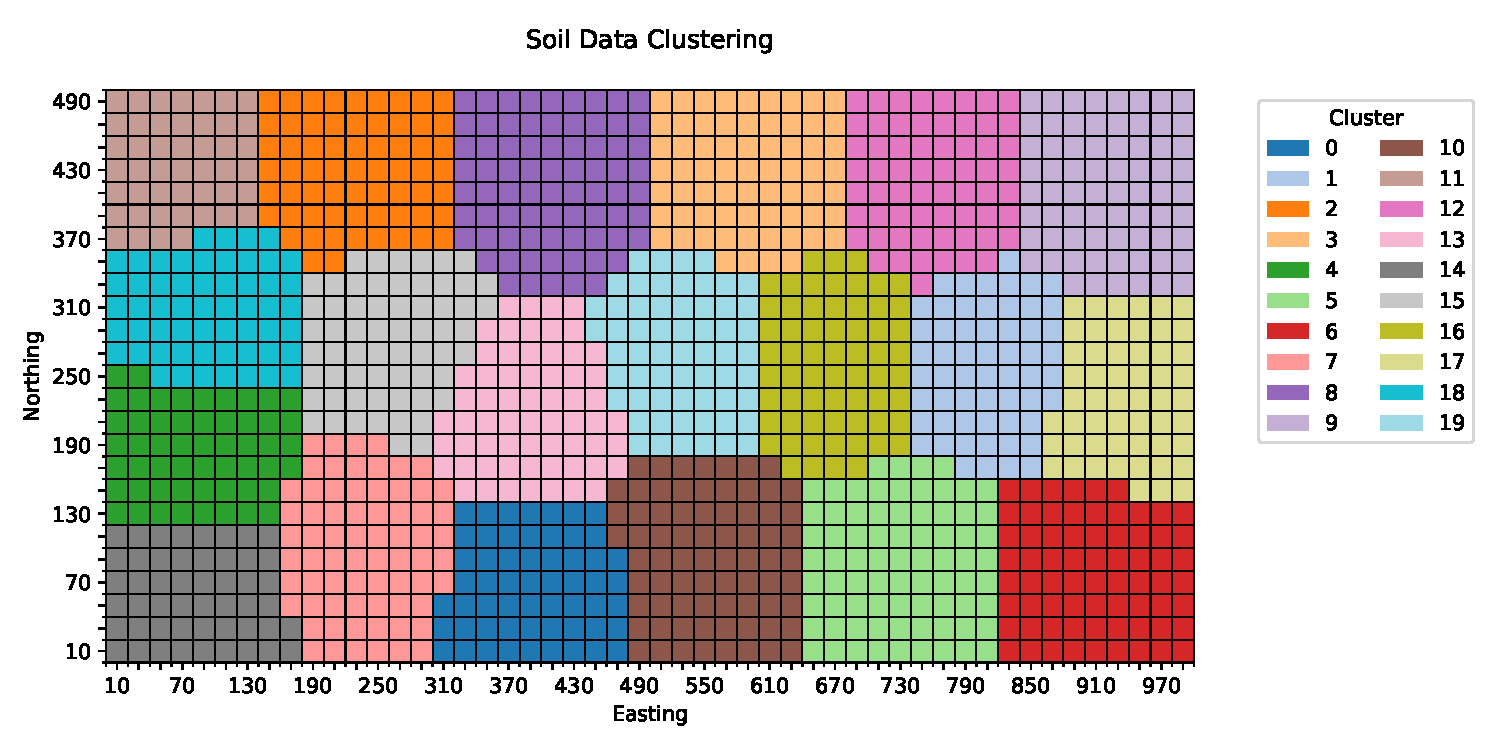
\includegraphics[width=\linewidth]{img/clusters_A.pdf}
    \caption{Distribution of clusters}
    \label{fig:clusters_A}
\end{figure}

\begin{figure}
    \centering
    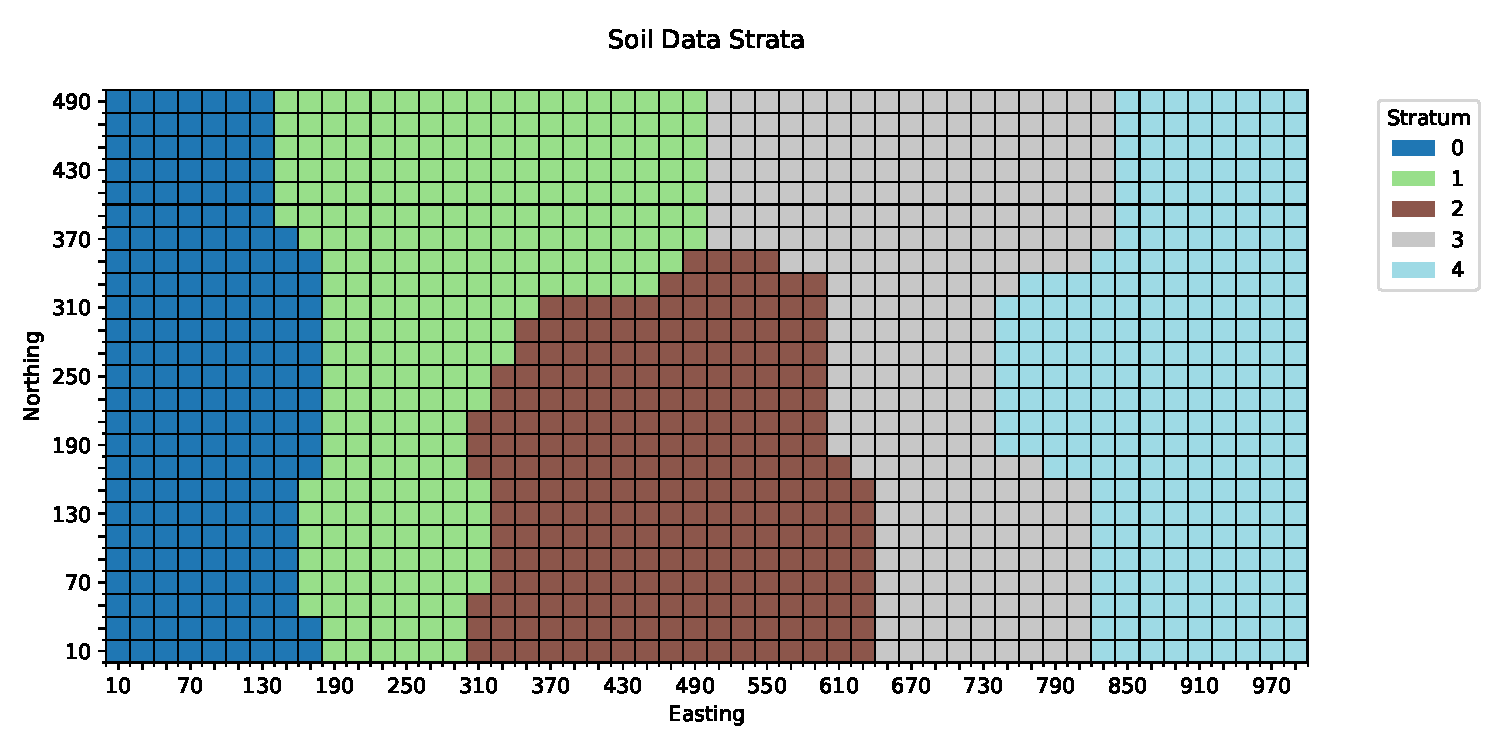
\includegraphics[width=\linewidth]{img/simple_strata.pdf}
    \caption{Distribution of strata}
    \label{fig:simple_strata}
\end{figure}


\subsection{Two-stage cluster random sampling -- probability proportional to size}\label{subsection_A}
    In this part, we are first selecting clusters with probabilities proportional to the sample sizes (with replacement); the selected clusters can be seen in Figure~\ref{fig:selected_clusters_A}.  (Note, in this particular example, we were "lucky" and did not have any cluster selected more than once, but it can happen in this setting.) The following clusters were selected: $2, 3, 5, 7, 16, 18$.

    From those clusters, we are sampling individual units. The random sample can be seen in Figure~\ref{fig:selected_points_A}.
    To illustrate, we will name selected points from one cluster (cluster $18$) displayed in light blue. We have selected population units displayed in Table~\ref{tab:points_A}. From the table, we can easily calculate that the sample mean for this particular cluster is: $\hat{m}(z)_{18} = 6574.4$.
    
\begin{table}[h]
\centering
\begin{tabular}{|c|c|c|}
\hline
$x$ & $y$ & $Cu$ \\
\hline
30 & 350 & 6400 \\
70 & 310 & 7051 \\
90  & 370 & 7007 \\
30 & 310 & 6252\\
30  & 330 & 6162 \\
\hline
\end{tabular}
\caption{$x$, $y$, and $Cu$ values for selected points in cluster $18$ -- probability proportional to size}
\label{tab:points_A}
\end{table}


\begin{figure}
    \centering
    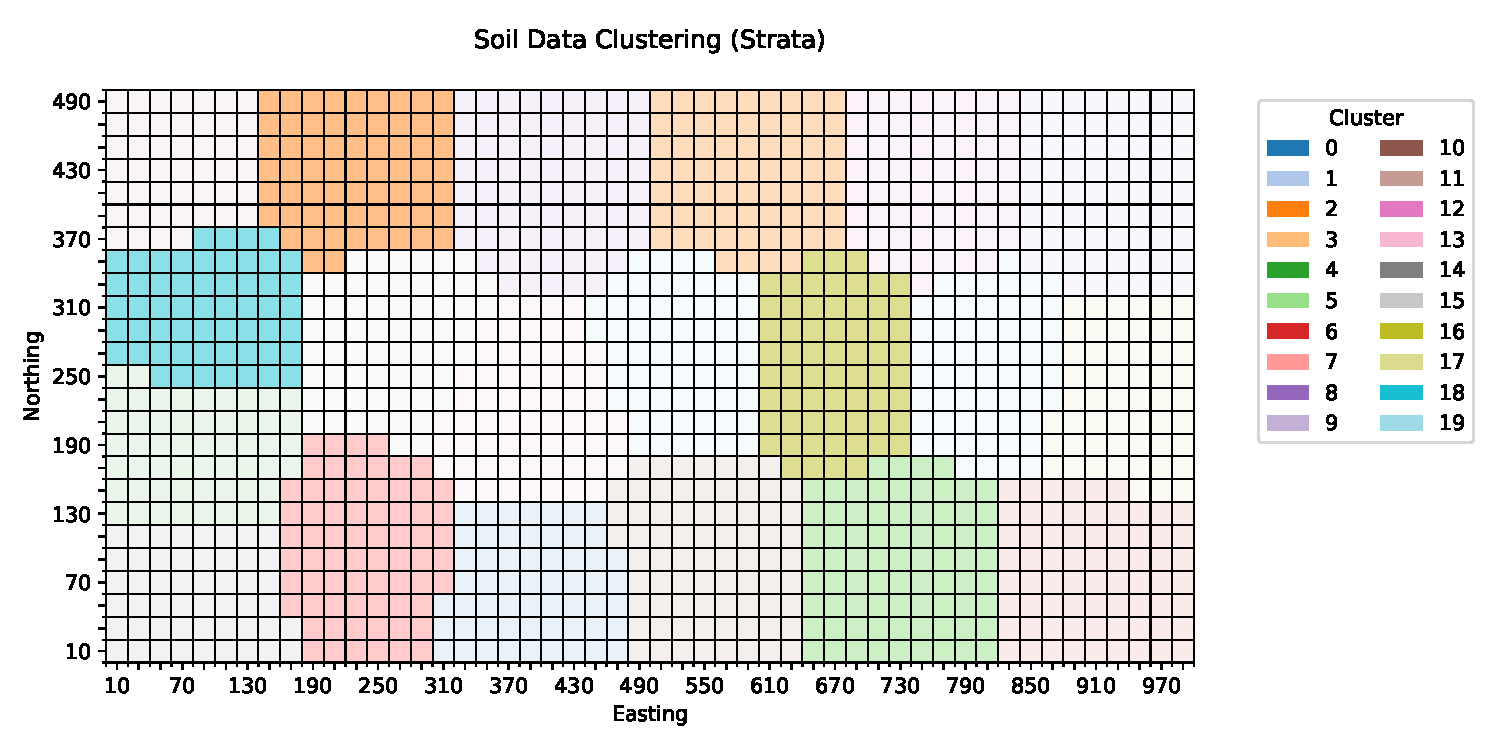
\includegraphics[width=\linewidth]{img/selected_clusters_A.pdf}
    \caption{Selected clusters (highlighted) - probability proportional to size}
    \label{fig:selected_clusters_A}
\end{figure}

\begin{figure}
    \centering
    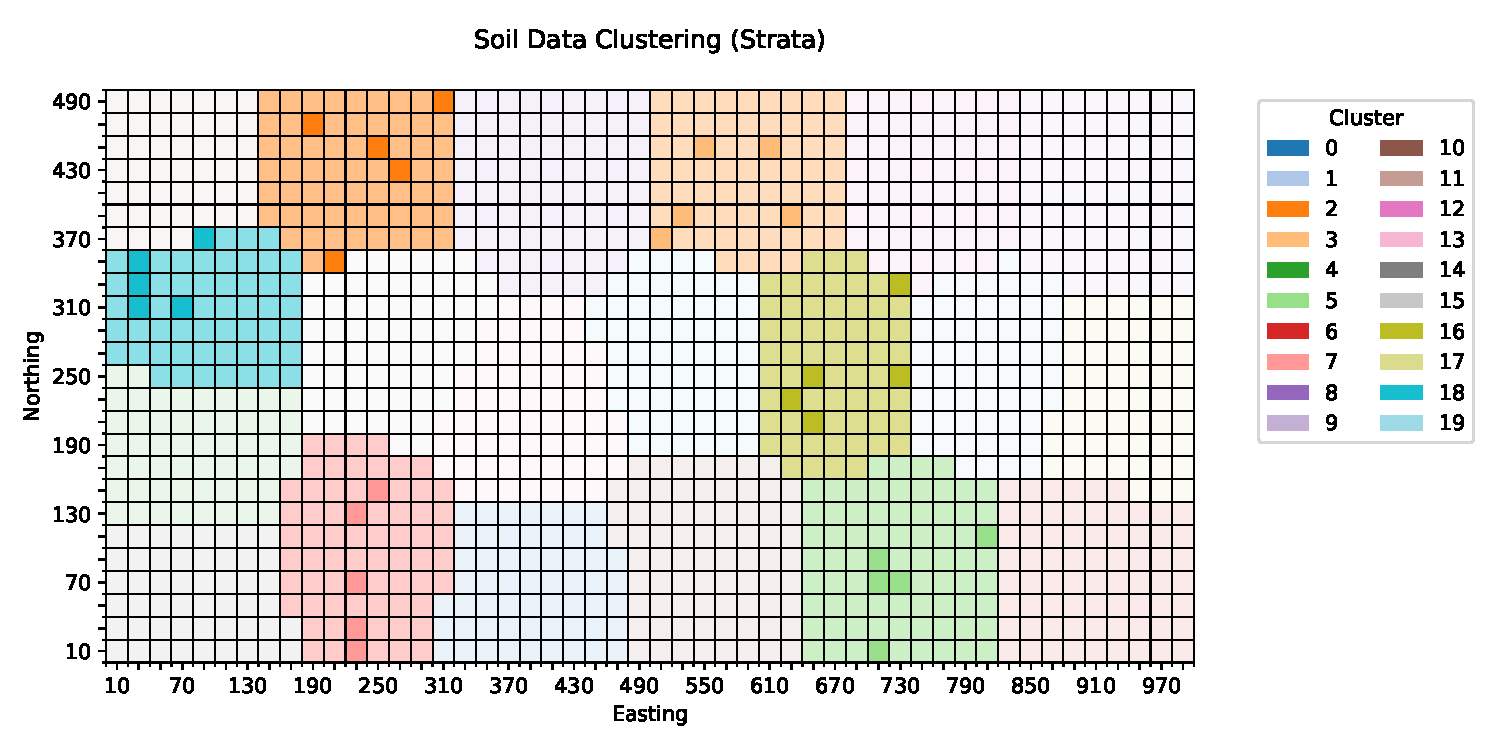
\includegraphics[width=\linewidth]{img/selected_points_A.pdf}
    \caption{Selected population points in clusters (highlighted) -- probability proportional to size}
    \label{fig:selected_points_A}
\end{figure}

In this particular setting, we get that the sample mean $\hat{m}(z)_{cl2(PP)}=7009.67$ and sample variance $\hat{var}(z)_{cl2(PP)}=258130.64$. We used the following formulae (both taken from \cite{thompson2012sampling}): 
\[
    \hat{t}(z)_{cl2(PP)}=\frac{M}{n_{psu}} \sum_{j \in \mathcal{S}} \frac{\hat{t}(z)_{j}}{M_j}=\frac{M}{n_{psu}}\sum_{j \in \mathcal{S}} \hat{m}(z)_{j},
\]
from which we simply get that 
\[
    \hat{m}(z)_{cl2(PP)}=\frac{1}{n_{psu}} \sum_{j \in \mathcal{S}} \frac{\hat{t}(z)_{j}}{M_j}=\frac{1}{n_{psu}}\sum_{j \in \mathcal{S}} \hat{m}(z)_{j}.
\]

For the sample variance, we use the formula:
\[
     \hat{var}(\hat{m}(z)_{cl2(PP)}) = \frac{1}{n_{psu}(n_{psu}-1)}\sum_{j \in \mathcal{S}} \left(\hat{m}(z)_j - \hat{m}(z)_{cl2(PP)} \right)^2.
\]


\subsection{Two-stage cluster random sampling -- simple random sampling}\label{subsection_B}
In this part, we first select clusters with uniform probabilities (simple random sampling); you can see selected clusters in Figure~\ref{fig:selected_clusters_B}. The following clusters were selected: $1, 2, 6, 16, 17, 18$  

From those clusters, we are sampling individual units. The random sample can be seen in Figure~\ref{fig:selected_points_B}. Let us again have a look at one specific cluster. Again, for cluster $18$, we have selected population units displayed in Table~\ref{tab:points_B}. In this case, we get that the sample mean is $\hat{m}(z)_{18}=6899.6$.



\begin{table}[h]
\centering
\begin{tabular}{|c|c|c|}
\hline
$x$ & $y$ & $Cu$ \\
\hline
130 & 290 & 7306 \\
130 & 270 & 6899 \\
90 & 290 & 7182 \\
50  & 250 & 6811 \\
150  & 270 & 6300 \\
\hline
\end{tabular}
\caption{$x$, $y$, and $Cu$ values for selected points in cluster $18$ -- simple random sampling}
\label{tab:points_B}
\end{table}

\begin{figure}
    \centering
    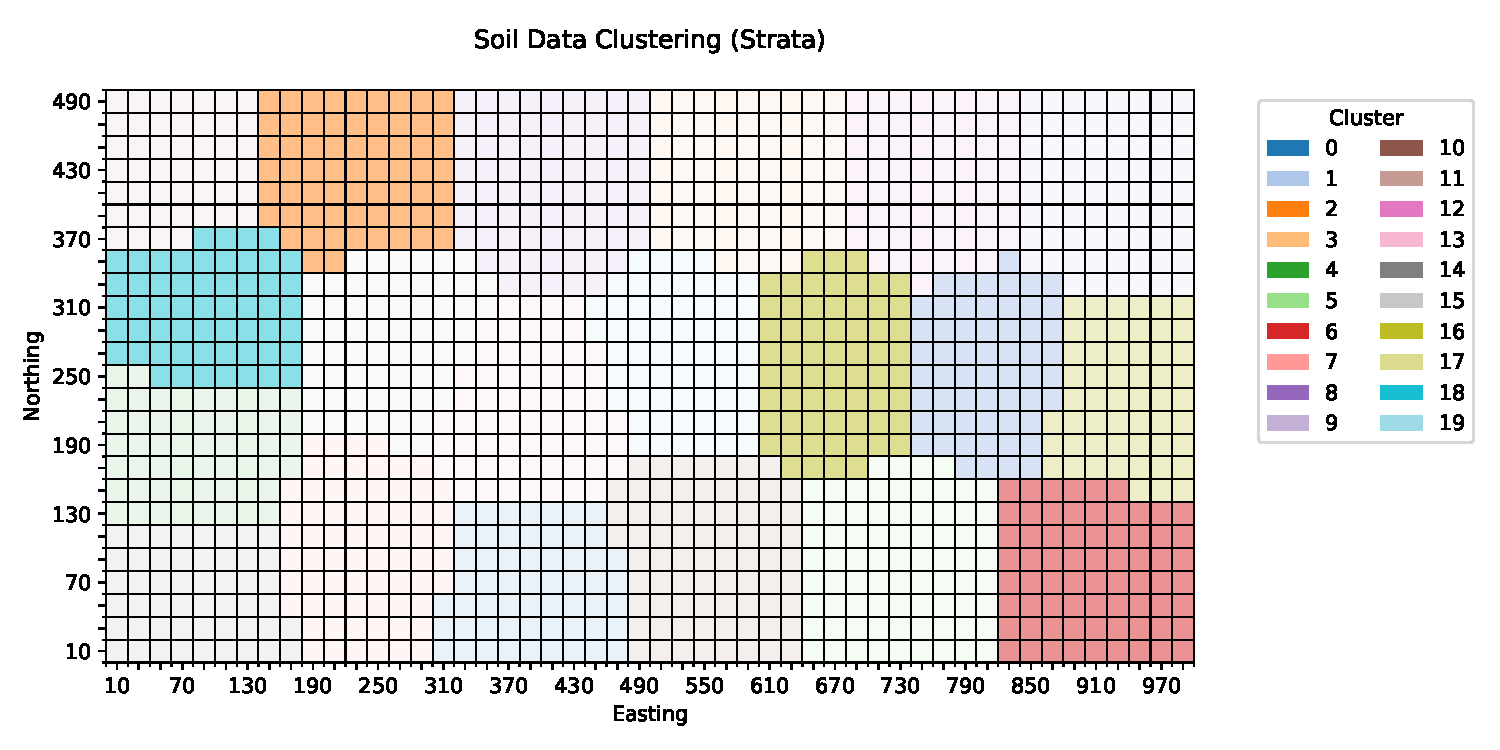
\includegraphics[width=\linewidth]{img/selected_clusters_B.pdf}
    \caption{Selected clusters (highlighted) -- simple random sampling}
    \label{fig:selected_clusters_B}
\end{figure}

\begin{figure}
    \centering
    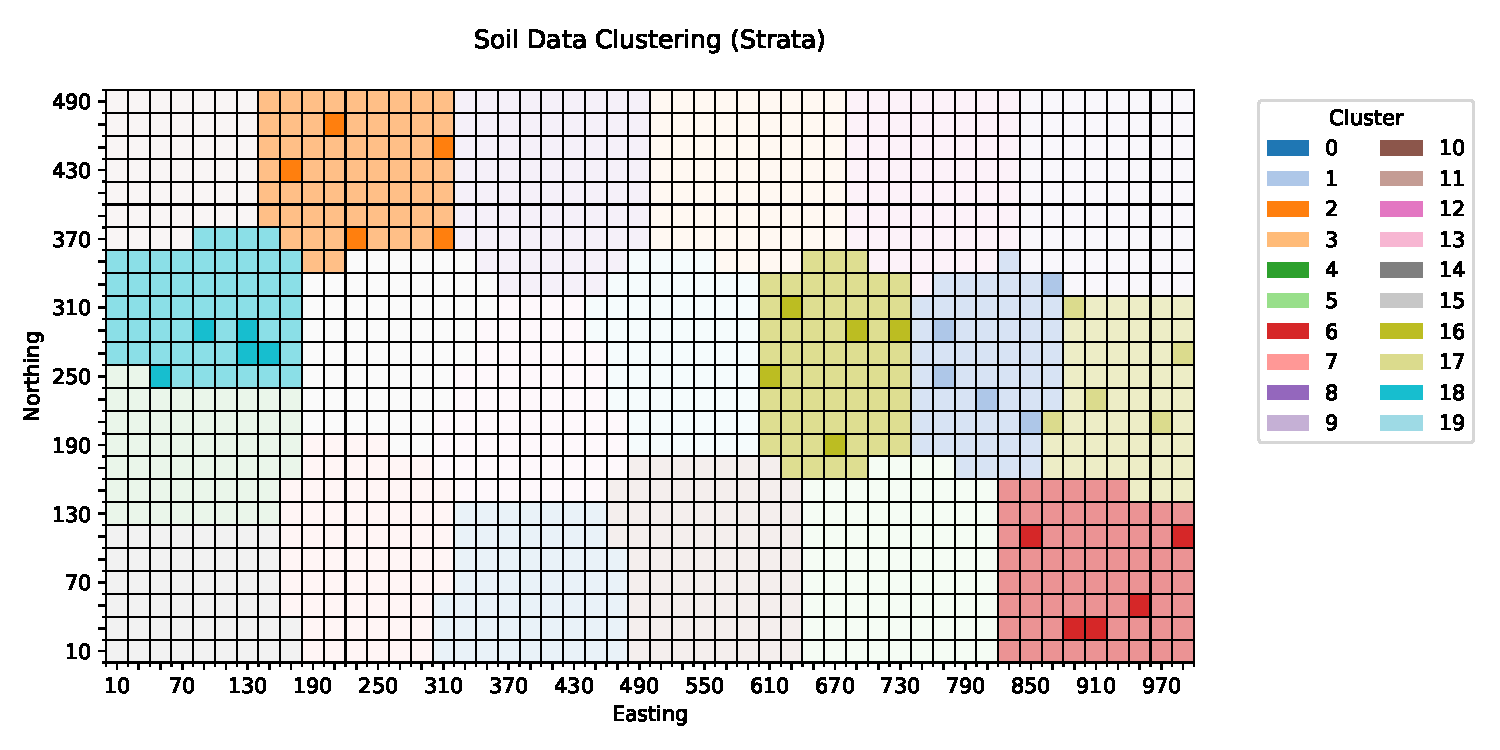
\includegraphics[width=\linewidth]{img/selected_points_B.pdf}
    \caption{Selected population points in clusters (highlighted) -- simple random sampling}
    \label{fig:selected_points_B}
\end{figure}
We calculated that the sample mean $\hat{m}(z)_{cl2(SI)} =7775.76 $ and sample variance $\hat{var}(\hat{m}(z)_{cl2(SI)}) = 345670.87$.
We used the following formulae (again taken from \cite{thompson2012sampling}):
\[
    \hat{t}(z)_{cl2(SI)} = \sum_{j \in \mathcal{S}} \frac{\hat{t}(z)_j}{\pi_j} = \frac{N}{n_{psu}} \sum_{j \in \mathcal{S}} \hat{t}(z)_j ,
\]
 where $\pi_j$ is the inclusion probability that is: $\pi_j = \frac{n_{psu}}{N}$ for $j \in \{1,2,, \ldots, N \}$ and consequently 
\[
    \hat{m}(z)_{cl2(SI)} = \frac{\hat{t}(z)_{cl2(SI)}}{M} = \frac{n_{psu}}{N M} \sum_{j \in \mathcal{S}} \hat{t}(z)_j.
\]

For the sample variance of the total's estimator, we use the formula:

\[
     \hat{var}(\hat{t}(z)_{cl2(SI)}) = N(N-n_{psu})\frac{s_u^2}{n_{psu}} + \frac{N}{n_{psu}}\sum_{j \in \mathcal{S}} M_j(M_j-m_j) \frac{s_j^2}{m_j},
\]

where 
\[
    s_u^2 = \frac{1}{n_{psu}-1}\sum_{j \in \mathcal{S}}\left(\hat{t}(z)_j - \hat{t}(z)\right)^2
\]

and $s_j^2$ is the within--cluster $j$ variance:
\[
    s_j^2 = \frac{1}{m_j-1} \sum_{i \in \mathcal{S}_j} \left( z_i - \hat{m}(z)_j\right)^2.
\]

If we divide by $M^2$, we get the formula for the sample variance of the mean's estimator: 
\[
     \hat{var}(\hat{m}(z)_{cl2(SI)}) = \frac{N(N-n_{psu})\frac{s_u^2}{n_{psu}} + \frac{N}{n_{psu}}\sum_{j \in \mathcal{S}} M_j(M_j-m_j) \frac{s_j^2}{m_j}}{M^2},
\]

\subsection{Stratified two-stage cluster random sampling}\label{subsection_C}
To explain the naming. We select clusters by stratified cluster random sampling, then in each stratum we select clusters by simple random sampling, and in each cluster we select population units again by simple random sampling. 

Let us now list the strata and corresponding selected clusters: $0: 14,18$, $1:7,8$, $2:13,19$, $3:5,12$, $4:9,17$. Our calculations now are very similar to the calculations in the previous section. We look at each strata individually and calculate the sample mean and sample variance and weigh them.
The selected population points can be seen in Figure~\ref{fig:selected_points_C}


\begin{figure}
    \centering
    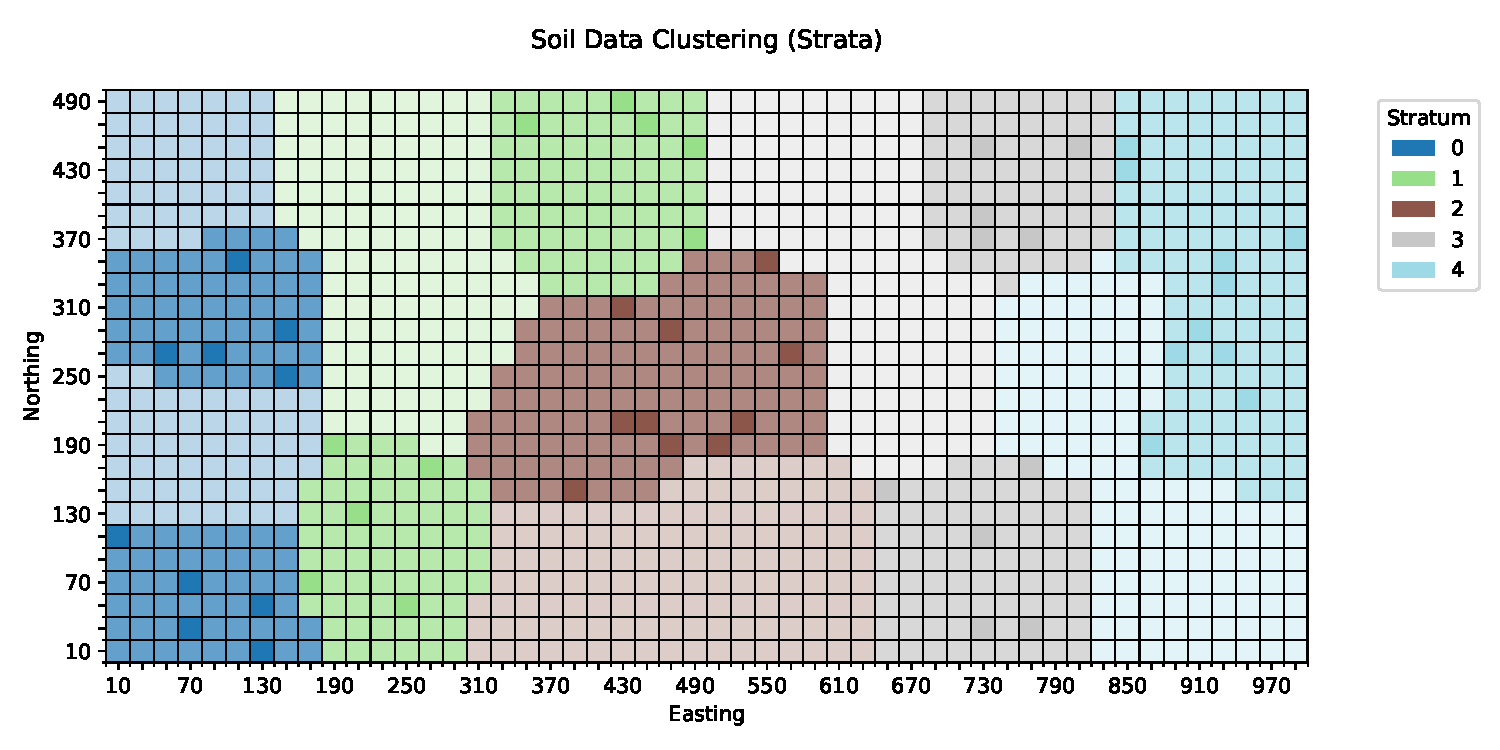
\includegraphics[width=\linewidth]{img/selected_points_C.pdf}
    \caption{Selected population points in clusters (highlighted) -- stratified version}
    \label{fig:selected_points_C}
\end{figure}

For the population total, it holds:
\[
    \hat{t}(z)_{st} = \sum_{h=1}^{N_{strata}} \hat{t}_h,
\]

where $\hat{t}_h$ is the population total estimator of stratum $h$.

Thanks to the independence of selections in different strata, the sample variance is the sum of the sample variances of individual stratum estimators: 
\[
    \hat{var}(\hat{t}_{st}) = \sum_{h=1}^{N_{strata}} \hat{var}(\hat{t}_h).
\]

From these formulae we easily get to $\hat{m}(z)_{st} = \frac{1}{M}\hat{t}(z)_{st}$ and $\hat{var}(\hat{m}_{st}) = \frac{1}{M^2} \hat{var}(\hat{t}_{st})$.

We got the following sample mean and variance: $\hat{m}(z)_{st} = 7525.21$ and $\hat{var}(\hat{m}_{st}) = 126089.89$.

\subsection{Simple random sampling of the population units} \label{subsection_D}
Here, we simply take simple random samples of the population units without replacement. The sample mean is calculated via:
\[
    \hat{m}(z) = \frac{1}{n_D} \sum_{j \in \mathcal{S}} z_j
\]

and sample variance of the mean's estimator:
\[
    \hat{var}(\hat{m}(z)) = \left(1-\frac{n_D}{M}\right) \frac{1}{n_D} \frac{1}{n_D-1} \sum_{j \in \mathcal{S}} \left(z_j - \hat{m}(z) \right)^2.
\]

Overall, we get that the sample mean is $7170.83 $ and the sample variance is $112711.91$.


\begin{figure}
    \centering
    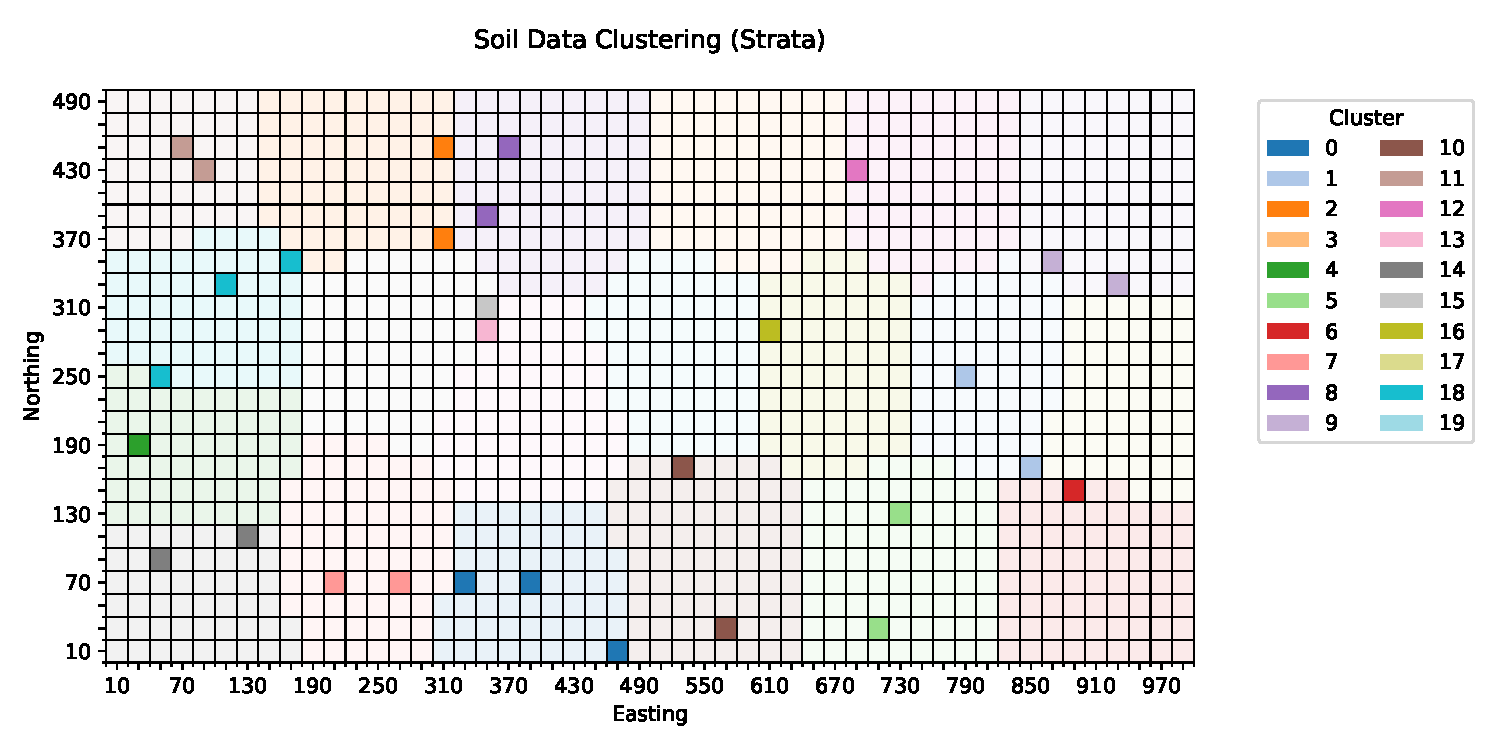
\includegraphics[width=1\linewidth]{img/selected_points_D.pdf}
    \caption{Selected population points by simple random sampling}
    \label{fig:selected_points_D}
\end{figure}
\section{Data analysis}
In this part, we will have a look at the estimated means and variances among several combinations of sample sizes and percentages of white pixels. We will keep the same clusters and strata we have been using in the previous section. 
We will provide three tables for different percentages of white pixels, ranging from $0$ to $0.5$. We will use varying $n_{psu}$,  $n_{ssu}$, and $N_{CinS}$ and display the values in the tables.
Additional updated data rows for ssu=2 (added to respective tables)
\begin{table}[htbp]
\centering
\begin{tabular}{rrrrrrrrrrr}
\hline
psu & ssu & CinS & A\_mean & A\_variance & B\_mean & B\_variance & C\_mean & C\_variance & D\_mean & D\_variance \\
\hline
10 & 2 & 2 & 7075.75 & 235324.54 & 7364.68 & 527705.56 & 6433.79 & 171740.31 & 7234.00 & 342764.33 \\
10 & 5 & 2 & 7600.90 & 158032.47 & 7393.57 & 232862.58 & 7387.62 & 187493.68 & 7134.58 & 60141.68 \\
10 & 10 & 2 & 6532.98 & 252517.61 & 7270.80 & 240312.02 & 6806.22 & 106901.10 & 7147.07 & 38061.70 \\
15 & 2 & 3 & 6795.13 & 115639.01 & 7114.02 & 114641.68 & 6915.90 & 46405.99 & 6974.53 & 188855.33 \\
15 & 5 & 3 & 7087.52 & 126584.87 & 7146.36 & 85899.40 & 6829.02 & 48172.16 & 7047.09 & 61819.29 \\
15 & 10 & 3 & 6964.38 & 155253.65 & 6617.94 & 58021.13 & 7160.75 & 42001.39 & 7117.59 & 21317.41 \\
\hline
\end{tabular}
\caption{Data for percentage of white pixels 0.0}
\label{tab:white_0}
\end{table}

% For percentage_white_pixels = 0.1
\begin{table}[htbp]
\centering
\begin{tabular}{rrrrrrrrrrr}
\hline
psu & ssu & CinS & A\_mean & A\_variance & B\_mean & B\_variance & C\_mean & C\_variance & D\_mean & D\_variance \\
\hline
10 & 2 & 2 & 7664.80 & 369982.62 & 6495.03 & 241991.81 & 7375.85 & 145130.49 & 6956.30 & 167079.71 \\
10 & 5 & 2 & 6603.90 & 151990.10 & 7831.85 & 233283.21 & 7002.73 & 124543.53 & 7144.84 & 53823.86 \\
10 & 10 & 2 & 7022.49 & 165232.83 & 7288.44 & 196437.64 & 6949.38 & 143750.24 & 6929.29 & 36463.14 \\
15 & 2 & 3 & 6539.73 & 204956.02 & 7329.96 & 160624.35 & 6923.06 & 83050.36 & 6837.00 & 114240.36 \\
15 & 5 & 3 & 7055.09 & 262360.03 & 7187.04 & 121979.54 & 7015.31 & 60987.07 & 6857.25 & 51619.05 \\
15 & 10 & 3 & 6835.23 & 123077.25 & 7292.22 & 87239.48 & 6911.44 & 13356.38 & 7084.49 & 26223.76 \\
\hline
\end{tabular}
\caption{Data for the percentage of white pixels 0.1}
\label{tab:white_0.1}
\end{table}

% For percentage_white_pixels = 0.5
\begin{table}[htbp]
\centering
\begin{tabular}{rrrrrrrrrrr}
\hline
psu & ssu & CinS & A\_mean & A\_variance & B\_mean & B\_variance & C\_mean & C\_variance & D\_mean & D\_variance \\
\hline
10 & 2 & 2 & 6867.90 & 286351.15 & 5836.61 & 224446.58 & 7606.69 & 198813.67 & 6462.75 & 98269.86 \\
10 & 5 & 2 & 6817.78 & 185692.39 & 7366.55 & 275946.83 & 7129.00 & 194124.45 & 6840.04 & 52567.15 \\
10 & 10 & 2 & 7302.55 & 100786.94 & 6573.93 & 189065.89 & 7393.03 & 75696.76 & 6949.28 & 38037.48 \\
15 & 2 & 3 & 7316.00 & 49999.13 & 6921.88 & 206632.99 & 7269.64 & 65239.99 & 7428.27 & 130347.42 \\
15 & 5 & 3 & 6717.33 & 98053.35 & 6735.56 & 106104.59 & 6979.44 & 46539.87 & 7240.03 & 53324.39 \\
15 & 10 & 3 & 6833.83 & 165710.57 & 7314.51 & 75032.24 & 6903.91 & 46504.60 & 6924.14 & 17788.90 \\
\hline
\end{tabular}
\caption{Data for the percentage of white pixels 0.5}
\label{tab:white_0.5}
\end{table}

% Table for percentage_white_pixels = 0.0

In all three tables (\ref{tab:white_0}, \ref{tab:white_0.1}, \ref{tab:white_0.5}) we have columns \texttt{psu} which is the number of primary sampling units in \ref{subsection_A} and \ref{subsection_B}. In \ref{subsection_C} we select \texttt{CinS} clusters per stratum. In each cluster, we select \texttt{ssu} secondary (population units). In \ref{subsection_D} we sample $\texttt{psu} * \texttt{ssu}$ population units.

Let's first have a look at the case when the percentage of white pixels is zero (Table~\ref{tab:white_0}). If we have a look at the sampling variances, we can see that the sampling variance is usually the lowest in stratified two-stage cluster random sampling. 

We can generally see that the variance in $D$ is lowest for higher numbers of selected secondary units, while the variance in $ C$ is lowest for lower numbers of selected secondary units.


In Table~\ref{tab:white_0.1} (referring to the sample means and variances of those estimators when the percentage of white points is $0.1$), we can see that the variances in $A$ and $B$ are much higher than the variances in $C$ and $D$. When we compare the latter two variances, we see that for lower $ssu$ the variance is lower in $C$ and otherwise the variance in $D$ is lower. We do not see any big difference in variances with different percentages of white points.

In Table~\ref{tab:white_0.5} (referring to the sample means and variances of those estimators when the percentage of white points is $0.5$,) we see similar behavior. Variances in $A$ and $B$ are much higher. However, $D$ is superficial to $C$ with the only significant difference when $psu=15$, $ssu=2$, and $C_{in}S = 3$, otherwise $D$ has much lower sample variance.



\section{Conclustion}
Our goal was to compare several sampling methods, specifically two-stage cluster random sampling. We concluded that the two approaches with plain two-stage cluster random sampling (with probabilities proportional to sample size and with equal probabilities (simple random sampling) in the first stages perform much worse compared to simple random sampling of the population units and stratified two-stage cluster random sampling. Overall, we can say that simple random sampling performs better. However, at the expense of the sampling costs, which are commonly higher when compared to cluster random sampling at the same total size of sampled population units.



\clearpage
\FloatBarrier
\bibliographystyle{plain} % or try 'abbrv', 'alpha', 'ieeetr', etc.
\bibliography{references} % the filename of your .bib file, without extension



\end{document}
